\providecommand\lcode{\begingroup \small\urlstyle{tt}\Url}
\providecommand\lident{\begingroup \small\urlstyle{tt}\Url}

\chapter{Propagating Information using SSA\Author{F. Brandner, D. Novillo}}
\inputprogress
\newcommand{\obacht}[2]{\marginpar{\tiny\textbf{#1:} #2}}

\graphicspath{{img/}{constant_propagation_is_easier/img/}{part3/constant_propagation_is_easier/img/}}

\lstdefinelanguage{DNlisting}
{
  morekeywords={PHI,ASSERT_EXPR},
  morekeywords=[2]{struct,const,int,void,for,if,throw,call,return},
  sensitive=true,
%   morecomment=[s]{<!--}{-->},
%   morestring=[b]",
}

\lstset{
  mathescape=true,
  language=DNlisting,
  basicstyle=\small,
  keywordstyle=\ttfamily,
  keywordstyle=[2]\bfseries,
%   identifierstyle=,
%   stringstyle=\color{black}\ttfamily,
%   commentstyle=\it,
%   moredelim=[is][\color{MyDarkGreen}\ttfamily]{|}{|}
  numbers=left
}

\section{Overview}

A central task of compilers is to \emph{optimize} a given input program such
that the resulting code is more efficient in terms of execution time, code size,
or some other metric of interest. However, in order to perform optimizations and
program transformations typically some form of \emph{program analysis} is
required in order to determine if a given transformation is applicable, to
estimate its profitability, or guarantee correctness.

\emph{Data flow analysis}~\cite{novillo:bib:NNH99} is a simple, yet powerful,
approach to program analysis that is utilized by many compiler frameworks and
program analysis tools today. We will introduce the basic concepts of
traditional data flow analysis in this chapter and show that \emph{static single
assignment} form (SSA) facilitates the design and implementation of equivalent
analyses, while leveraging properties of programs in SSA form allows to reduce
the compilation time and memory consumption.

Traditionally, data flow analysis is performed on a \emph{control flow graph}
(CFG) representation of the input program, where nodes in the graph represent
operations and edges the possible flow of program execution.
Information on certain \emph{program properties} is propagated among
the nodes along the control flow edges until the computed information at the
nodes stabilizes, i.e., no \emph{new} information can be devised from the
program.

The \emph{propagation engine} presented in the following sections is an
extension of the well known approach by Wegman and Zadeck for \emph{sparse
conditional constant propagation}~\cite{bib:wegman.ea-91} (also known as
SSA-CCP). Instead of using the CFG they represent the input program as an
\emph{SSA graph}~\cite{novillo:bib:cytron.ea-91}. Operations are again represented as
nodes in this graph, however, the edges represent \emph{data dependencies}
instead of control flow. This representation allows a selective propagation of
program properties among data dependent graph nodes only. As before, the
processing stops when the information at the graph's nodes stabilizes. The basic
algorithm is not limited to constant propagation and can also be applied to
solve a large class of other data flow problems
efficiently~\cite{novillo:bib:N05}. However, not all data flow
analyses can be modeled. We will thus investigate the limitations
of the SSA-based approach and briefly discuss problems that
cannot be modeled.

The remainder of this chapter is organized as follows. First, the basic concepts
of (traditional) data flow analysis are presented in
Section~\ref{novillo:sec:preliminaries}. This will provide the theoretical
foundation and background for the discussion of the SSA-based propagation
engine in Section~\ref{novillo:sec:prop-engine}. We then provide examples of
data flow analyses that can be realized efficiently by the aforementioned
engine, namely copy propagation in Section~\ref{novillo:sec:copy-prop} and value
range propagation in Section~\ref{novillo:sec:vrp}. Finally, some examples of
data flow problems are given that cannot be modeled using the generic
propagation engine but still benefit from SSA properties in
Section~\ref{novillo:sec:beyond_sparse_data_propagation}. We conclude and
provide links for further reading in Section~\ref{novillo:sec:further_reading}.

%%%%%%%%%%%%%%%%%%%%%%%%%%%%%%%%%%%%%%%%%%%%%%%%%%%%%%%%%%%%%%%%%%%%%%%%%%%%%%%%
\section{Preliminaries}
\label{novillo:sec:preliminaries}

Data flow analysis is at the heart of many compiler transformations and
optimizations, but also finds application in a broad spectrum of analysis and
verification tasks in program analysis tools such as program checkers, profiling
tools, and timing analysis tools. This section gives a brief introduction to the
basics of data flow analysis, due to space considerations, we cannot cover this
topic in full depth.

As noted before, data flow analysis allows to derive information of certain
interesting program properties that may help to optimize the program. Typical
examples of interesting properties are: The set of \emph{live} variables at a
given program point, the constant value a variable may take, or the set of
program points that are reachable at run-time. Liveness information is critical,
for example, during register allocation, while the two latter properties help
in simplifying computations and avoiding useless calculations as well as dead
code.

The analysis results are gathered from the input program by propagating
information among its operations along all possible execution paths. The
propagation is typically performed iteratively until the computed results
stabilize. Formally, a data flow problem can be specified using a \emph{monotone
framework} that consists of:
\begin{itemize}
  \item a \emph{complete lattice} representing the property space,
  \item a \emph{flow graph} resembling the control flow of the input program,
  \item and a set of \emph{transfer functions} modeling the effect of individual
        operations \\ on the property space.
\end{itemize}

%///////////////////////////////////////////////////////////////////////////////
\subsection{Property Space}
\label{novillo:sec:property_space}

\begin{figure}[t]
  \begin{center}
    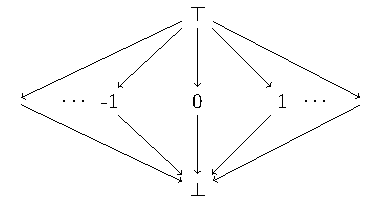
\includegraphics{constprop_lattice}
  \end{center}
  \vspace{-1em}
  \caption{Example of a lattice, which is commonly used to represent whether a
           variable is known to hold a constant value at a given program point.}
  \label{novillo:fig:lattice_constant_propagation}
\end{figure}

A key concept for data flow analysis is the representation of the property
space via \emph{partially ordered sets}. A partially ordered set $(L,
\sqsubseteq)$ is a set $L$ that is equipped with a reflexive, transitive, and
anti-symmetric relation $\sqsubseteq\colon L \times L \rightarrow \{true, false\}$.
Based on the relation an \emph{upper bound} for subsets of $L$ can be defined:
$l \in L$ is the upper bound for a subset $Y$ of $L$ if $\forall l' \in Y\colon l'
\sqsubseteq l$. Furthermore, $l \in L$ is the \emph{least upper bound} if it is
an upper bound and for any other upper bound $l_o$ of $Y$: $l \sqsubseteq l_0$.
Lower bounds and greatest lower bounds are defined analogously.

A particularly interesting class of partially ordered sets are \emph{complete
lattices}, where all subsets have a least upper bound as well as a greatest
lower bound. These bounds are unique and are denoted by $\bigsqcup$ and
$\bigsqcap$ respectively. In the context of program analysis the former is often
referred to as the \emph{join operator}, while the latter is termed the
\emph{meet operator}. Complete lattices have two distinguished elements, the
\emph{least element} and the \emph{greatest element}, often denoted by $\bot$
and $\top$ respectively.

An \emph{ascending chain} is a totally ordered subset $\{l_1, \ldots, l_n \}$ of
a complete lattice, where for all $i, j \in \{1, \ldots, n\}, i < j \colon l_i
\sqsubseteq l_j$. A chain is said to \emph{stabilize} if there exists an $i_0
\in \mathbb{N}$, where $\forall i \in \mathbb{N}, i > i_0 \colon l_i = l_{i_0}$;
$i_0$ is then called the \emph{length} of the chain.

Consider, for example, the lattice presented in
Figure~\ref{novillo:fig:lattice_constant_propagation} that is commonly used to
represent whether a given variable is known to hold a specific constant value at
a given program point at run-time. The analysis and the corresponding
optimization are often uniformly referred to as \emph{constant propagation}.
For this lattice, $\top$ indicates that no specific information on the
variable's value is available. The symbol $\bot$, on the other hand, indicates
that the analysis was not able to prove that the variable holds the same
constant value in all cases. The other elements in the lattice denote that the
variable is known to hold the respective value. The $\sqsubseteq$ relation is
represented by the arrows in the figure. Clearly, all chains for this lattice
are at most of length three ($\bot \sqsubseteq c \sqsubseteq \top$, $c \in
\mathbb{N}$).

%///////////////////////////////////////////////////////////////////////////////
\subsection{Program Representation}
\label{novillo:sec:program_representation}

\begin{figure}[b]
  \begin{center}
    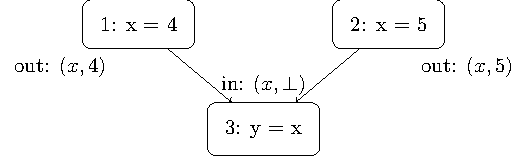
\includegraphics{contr_flow_graph}
  \end{center}
  \vspace{-1em}
  \caption{Combining data flow information using the join operator.}
  \label{novillo:fig:control_flow_graph}
\end{figure}

Individual functions of the input program are represented as separate flow
graphs of the form $G = (V,E)$, where the nodes represent operations, or
instructions, at a program point and edges denote the possible flow of control
at run-time. The graph contains two distinguished nodes, the \emph{start} node
$s$ and the \emph{exit} node $t$. These two nodes are special in that the former
is the only node without any predecessors and the latter is the only node
without any successors.

During the analysis, data flow information is propagated from one node to
another adjacent node along the respective graph edge. Every node is associated
with data flow information using two sets, \emph{in} and \emph{out}. If the
target node has a single incoming edge only, the propagation corresponds to a
simple copy from the source node's \emph{out} set to the target node's \emph{in}
set. However, in the more general case of multiple incoming edges, we need to
combine the information from all those edges. This is accomplished by applying
the join or meet operator of the lattice that represents the property space. For
example, consider the lattice from
Figure~\ref{novillo:fig:lattice_constant_propagation} and the flow graph shown
in Figure~\ref{novillo:fig:control_flow_graph}. We can clearly say that, after
executing operation $1$ on the top left side, variable x holds the
constant value of $4$, as indicated by the \emph{out} annotation $(x, 4)$ below.
The same applies for operation $2$ on the right, with the slight difference that
the variable holds the value of $5$. Combining this information yields $4
\bigsqcap 5 = \bot$, i.e., x does not hold a constant value at program point 3.

In many cases it is helpful to reverse the flow graph to propagate information,
i.e., reverse the direction of the graph's edges. Analyses relying on this
reversed flow graph are termed \emph{backward analyses}, while those using the
regular flow graph are called \emph{forward analyses}. As shown before,
computing whether a variable holds a certain constant value is a forward
problem, while determining whether a computation is dead, i.e., not used, is a
typical backward problem.

%///////////////////////////////////////////////////////////////////////////////
\subsection{Transfer Functions}

\begin{table}[b]
  \begin{center}
    \begin{tabular}{lp{8mm}l}
      Operation                   & & Transfer Function                      \\ \hline
      x = $c$, $c \in \mathbb{N}$ & & $f_{x=c}(L) = L \setminus \{ (x, c') | (x, c') \in L \} \cup \{ (x, c) \}$ \\
      x = y                       & & $f_{x=y}(L) = L \setminus \{ (x, c') | (x, c') \in L \} \cup \{ (x, c) | (y,c) \in L\}$ \\
      x = $\ldots$                & & $f_{x=\ldots}(L) = L \setminus \{ (x, c') | (x, c') \in L \}$ \\
      $\ldots$                    & & $f_{\ldots}(L) = L$ \\ \hline
    \end{tabular}
  \end{center}
  \caption{A simplified set of transfer functions for constant propagation
           analysis.}
  \label{novillo:fig:transfer_functions}
\end{table}

Aside from the control flow, the effect of the program's operations
need to be accounted for during analysis. However, in contrast to the actual
execution, we are only interested in an abstract model of the operations'
effects with respect to the data flow information. Operations are thus mapped to
a set of abstract \emph{transfer functions} of the form $f_{op}\colon L \rightarrow
L$ that transform the information available from the \emph{in} set of the
respective flow graph nodes and store the result in the corresponding \emph{out}
set.

Continuing the example from before, a simple set of transfer functions can be
defined, as shown in Table~\ref{novillo:fig:transfer_functions}. Assignments to
variables invalidate the information that is available on that particular
variable, i.e., information is removed from the input set. However, in the case
of a copy operation or the assignment of a constant value, new information is
obtained, i.e., is appended to the input set. Care has to be taken that
previous information is properly invalidated. Other operations not modifying any
variable are associated with the identity function, i.e., all the information is
preserved.

%///////////////////////////////////////////////////////////////////////////////
\subsection{Solving Data Flow Problems}

Putting all those elements together, i.e., a complete lattice, a flow graph, and
a set of transfer functions, yields an instance of a monotone framework. Which,
in fact, describes a set of \emph{data flow equations} that need to be solved in
order to retrieve the analysis result. A very popular and intuitive way of
solving these equations is to compute the \emph{maximal fixed point} (MFP) using
an iterative work list algorithm. The work list contains operations that have
to be reevaluated by first combining the information form all their predecessors
in the flow graph, then applying their transfer function, and finally
propagating the obtained information to all successors by appending them to the
work list. The algorithm terminates when the data flow information stabilizes
and the work list becomes empty~\cite{novillo:bib:NNH99}.

It is obvious that a single flow edge can be appended several times to the
work list in the course of the analysis. It may even happen that an infinite
feedback loop prevents the algorithm from terminating. We are thus interested in
bounding the number a given edge is processed. Recalling the definition of
chains from Section~\ref{novillo:sec:property_space}, the \emph{height} of a
lattice is defined by the length of its longest chain. We can ensure termination
for lattices fulfilling the \emph{ascending chain condition}, which ensures that
the lattice has finite height. Given a lattice with finite height $h$ and a flow
graph $G=(V, E)$ it is easy to see that the MFP solution can be computed in
$O(|E| \cdot h)$ time, or, due to the fact that $|E| \leq |V|^2$, in $O(|V|^2
\cdot h)$. Note that the height of the lattice often depends on properties of
the input program, which might ultimately yield bounds worse than cubic in the
number of graph nodes. Furthermore, every node of the flow graph is associated
with an \emph{in} and an \emph{out} set, in order to store data flow
information and propagate preliminary analysis results to the neighbors in the
graph. The sets often contain information that is unrelated to the particular
nodes in question in order to ensure that the information is properly propagated
to all relevant program points.

For reducible flow graphs the order in which operations are processed by the
work list algorithm can be
optimized~\cite{novillo:bib:HU73,novillo:bib:KU76,novillo:bib:NNH99}, allowing
to derive tighter complexity bounds. However, relying on reducibility is
problematic, because flow graphs are often \emph{not} reducible even for proper
structured languages, e.g., reversed flow graphs of backward problems can be,
and in fact almost always are, irreducible even for programs with reducible flow
graphs. Furthermore, experiments have shown that the tighter bounds not
necessarily lead to improved compilation times~\cite{novillo:bib:CTK06}.

Apart from computing a fixed point, data flow equations can also be solved using
a more powerful approach called the \emph{meet over all paths} (MOP) solution.
Even though more powerful, computing the MOP solution is often harder to compute
or even undecidable~\cite{novillo:bib:NNH99}. Consequently, the MFP solution is
preferred in practice.

%%%%%%%%%%%%%%%%%%%%%%%%%%%%%%%%%%%%%%%%%%%%%%%%%%%%%%%%%%%%%%%%%%%%%%%%%%%%%%%%
\section{Propagation Using the SSA Form}
\label{novillo:sec:prop-engine}

SSA form allows to solve a large class of data flow problems more efficiently
than the standard fixed point solution presented previously. The basic idea is
to directly propagate information computed at the unique definition of a
variable to all its uses. Intermediate program points on regular control flow
paths from the definition to those uses are skipped, reducing memory consumption
and compilation time.

%///////////////////////////////////////////////////////////////////////////////
\subsection{Program Representation}

Programs in SSA form exhibit, aside from the regular operations of the original
program, special operations called $\phi$-operations, which are placed at join
points of the original CFG -- see Part~\ref{part:vanilla_ssa} of this book for
more information. In the following, we assume that possible many
$\phi$-operations are associated with the corresponding CFG nodes at those
join points.

\obacht{Reference for SSA graphs}{Point directly to a chapter in the book?}
Data flow analysis under SSA form relies on a specialized program
representation based on \emph{SSA
graphs}~\cite{novillo:bib:cytron.ea-91}, which
allows to simplify the propagation of data flow information. The nodes of an
SSA graph correspond to the operations of the program. In particular the
program's $\phi$-operations are represented by dedicated nodes in the SSA graph.
The edges of the graph connect the unique definition of a variable with all its
uses, i.e., an edge represents a true data dependence among two nodes.

An important property of SSA graphs is that they also capture, besides the data
dependencies, the \emph{relevant} join points of the program's CFG. A join point
is relevant for the analysis, whenever the value of two or more definitions may
reach a use by passing through that join. Due to the properties of SSA form, it
is ensured that a $\phi$-operation is placed at the join point and that the use
has been properly updated to refer to the respective $\phi$-operation. Other
join points can safely be ignored, because uses are guaranteed to receive the
same value on all paths due to the dominance property.

\begin{figure}[t]
  \begin{center}
    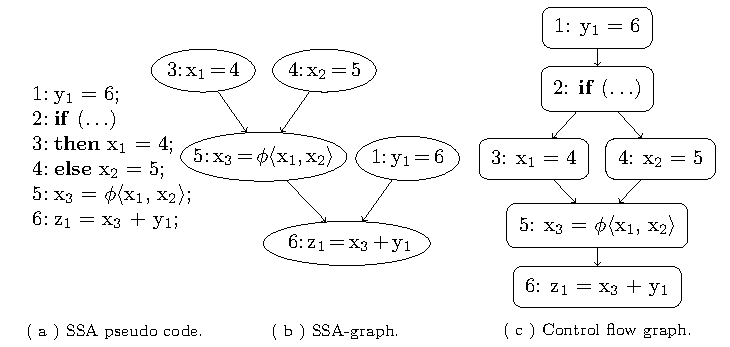
\includegraphics{ssa_graph}
  \end{center}
  \vspace{-2em}
  \caption{Example program and its SSA graph.}
  \label{novillo:fig:ssa_graph}
\end{figure}

Consider for example, the code excerpt shown in
Figure~\ref{novillo:fig:ssa_graph}, along with the corresponding SSA graph and
CFG. Assume we are interested in propagating information from the assignment of
variable y$_1$ at the beginning of the code excerpt down to its unique use at
the end. Using the traditional CFG representation this requires the propagation
to pass though several intermediate program points. These program points are
concerned with computations of the variables x$_1$  through x$_3$ only and are
thus irrelevant for the computation at hand. The SSA graph representation, on
the other hand, allows to propagate the desired information directly without any
intermediate steps. At the same time, we also find that the control flow join
following the \textbf{if} is properly represented by the $\phi$-operation
defining the variable x$_3$ in the SSA graph.

Even though the SSA graph captures data dependencies and the relevant join
points in the CFG, it lacks information on other
\emph{control dependencies}. However, analysis results can often be improved
significantly by considering the additional information that is available from
the control dependencies in the program's CFG. As an example consider once more
the code excerpt shown in Figure~\ref{novillo:fig:ssa_graph}. Assume that the
condition associated with the \textbf{if} operation is known to be false for all
possible program executions. Consequently, the $\phi$-operation will select the
value of x$_2$ in all cases, which is known to be of constant value $5$.
However, due to the shortcomings of the SSA graph this information cannot be
derived. It is thus important to use both graphs during data flow analysis
in order to obtain the best possible results.

%///////////////////////////////////////////////////////////////////////////////
\subsection{Sparse Data Flow Propagation}

\begin{algorithm}[t!]
  \begin{enumerate}
    \item Initially, every edge in the CFG is marked not executable and the
          \emph{FlowWorkList} is seeded with the outgoing edges of the flow
          graph's \emph{start} node.  The \emph{SSAWorkList} is empty.
    \item \label{novillo:alg:propagation:loop} Remove the top element of either
          of the two work lists.
    \item \label{novillo:alg:propagation:flowedge} If the element is a flow edge
          that is marked to be executable, do nothing, \\ otherwise proceed as
          follows:
          \begin{itemize}
            \item Mark the edge as executable.
            \item Visit every $\phi$-operation associated with the edge's target
                  node.
            \item When the target node was reached the first time via the
                  \emph{FlowWorkList} visit its operation.
            \item When the target node has a single outgoing non-executable edge
                  append that edge to the \emph{FlowWorkList}.
          \end{itemize}
    \item \label{novillo:alg:propagation:ssaedge} If the element is an edge from
          the SSA graph, process the target operation as follows:
          \begin{enumerate}
            \item[a.] When the target operation is a $\phi$-operation visit that
                      $\phi$-operation.
            \item[b.] \label{novillo:alg:propagation:ssaedge:regular} For
                      regular target operations, examine the corresponding
                      executable flag of the incoming edges of its corresponding
                      flow graph node. If any of those edges is marked
                      executable visit the operation, otherwise do nothing.
          \end{enumerate}
    \item Continue with step \ref{novillo:alg:propagation:loop} until both work
          lists become empty.
    \vspace{-1em}
  \end{enumerate}

  \caption{Sparse Data Flow Propagation}
  \label{novillo:alg:propagation}
\end{algorithm}

Similar to monotone frameworks for traditional data flow analysis, frameworks
for \emph{sparse data flow propagation} under SSA form can be defined. As
before, such a framework consist of: (1) a complete lattice, (2) a set of
transfer functions, (3) a flow graph, and, additionally, (4) an SSA graph. We
again seek a maximal fixed point solution (MFP) using an iterative work list
algorithm. However, in contrast to the algorithm described before, data flow
information is not propagated along the edges of the flow graph but along the
edges of the SSA graph. For regular uses the propagation is straightforward due
to the fact that every use receives its value from a unique definition. Special
care has to be taken for $\phi$-operations, which select a value among their
operands depending on the incoming flow edges. The data flow information of the
incoming operands has to be combined using the meet or join operator of the
lattice. As data flow information is propagated along SSA edges that have a
single source, is is sufficient to store the data flow information with the
node. The \emph{in} and \emph{out} sets used by the traditional approach -- see
Section~\ref{novillo:sec:program_representation} -- are obsolete, since
$\phi$-operations already provide the required buffering. Furthermore, the flow
graph is used in order to track which operations are not reachable under any
program execution and thus can be ignored safely during the computation of the
fixed point solution.

The algorithm processes two work lists, the \emph{FlowWorkList} containing edges
of the flow graph and the \emph{SSAWorkList}, which consists of edges from the
SSA graph. It proceeds by removing the top element of either of those lists and
processing the respective edge as indicated by
Algorithm~\ref{novillo:alg:propagation}. Throughout the algorithm operations of
the program may be visited in order to update the work lists and propagate
information as shown by Algorithm~\ref{novillo:alg:visit}. We will highlight
the most relevant parts of the algorithms in the following paragraphs and
explain some important aspects of their interaction.

\begin{algorithm}[t!]
  \begin{enumerate}
    \item Compute the operation's data flow information:
    \begin{enumerate}
      \item[a.] \label{novillo:alg:visit:phi} If the operation is a
                $\phi$-operation, combine the data flow information from all its
                operands where the corresponding flow edge is marked executable.
      \item[b.] \label{novillo:alg:visit:branch} In the case of conditional
                branches, update the operation's data flow information. Determine
                which of the outgoing flow edges are reachable from the
                corresponding flow graph node by examining the branch's
                condition(s) and append the respective non-executable edges to
                the \emph{FlowWorkList}.
      \item[c.] \label{novillo:alg:visit:regular} For regular operations, update
                the corresponding data flow information by applying its transfer
                function.
    \end{enumerate}
    \item Whenever the data flow information changes append all outgoing edges
          of the corresponding SSA graph node to the \emph{SSAWorkList}.
    \vspace{-1em}
  \end{enumerate}
  \caption{Visiting an Operation}
  \label{novillo:alg:visit}
\end{algorithm}

In step~\ref{novillo:alg:propagation:flowedge} of the main algorithm, flow edges
are processed that were encountered to be executable for the first time in the
course of the analysis. Whenever such a flow edge is processed, all
$\phi$-operations of its target node need to be reevaluated due to the fact that
Algorithm~\ref{novillo:alg:visit}a discarded the respective operands of the
$\phi$-operations so far -- because the flow edge was not yet marked executable.
Similarly, the operation of the target node has to be evaluated when the target
node is encountered to be executable for the first time, i.e., the currently
processed edge is the first of its incoming edges that is marked executable.
Note that this is only required the \emph{first} time the node is
encountered to be executable, due to the processing of operations in
Step~\ref{novillo:alg:propagation:ssaedge}b, which thereafter triggers the
reevaluation automatically when necessary.

Regular operations as well as $\phi$-operations are visited by
Algorithm~\ref{novillo:alg:visit} when the corresponding flow graph node has
become executable or whenever the data flow information of one of their
predecessors in the SSA graph changed. $\phi$-operations combine the information
from multiple flow paths using the usual meet operator, but only considering
those operands where the associated edge is marked executable. Conditional
branches are handled by examining its conditions based on the data flow
information computed so far. Depending on whether those conditions are
satisfiable or not, flow edges are appended to the \emph{FlowWorkList} in order
to ensure that all reachable operations are considered during the analysis.
Finally, all regular operations are processed by applying the relevant transfer
function and possibly propagating the updated information to all uses by
appending the respective SSA graph edges to the \emph{SSAWorkList}.

\begin{figure}[t!]
  \begin{center}
    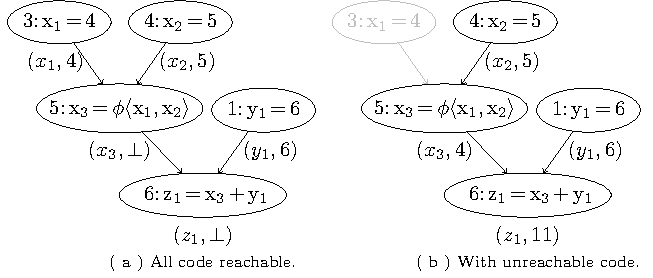
\includegraphics{ssa_propagation}
    \subfigure{\label{novillo:fig:ssa_propagation:a}}
    \subfigure{\label{novillo:fig:ssa_propagation:b}}
  \end{center}
  \vspace{-2em}
  \caption{Sparse data flow propagation using SSA graphs.}
  \label{novillo:fig:ssa_propagation}
\end{figure}

As an example, consider the program shown in Figure~\ref{novillo:fig:ssa_graph}
and the constant propagation problem. First,
assume that the condition of the \textbf{if} cannot be statically evaluated, we
thus have to assume that all its successors in the CFG are reachable.
Consequently, all flow edges in the program will eventually be marked
executable. This will trigger the evaluation of the constant assignments to
the variables x$_1$,  x$_2$, and y$_1$. The transfer functions immediately yield
that the variables are all constant holding the value $4$, $5$, and $6$
respectively. This new information will trigger the reevaluation of the
$\phi$-operation of variable x$_3$. As both of its operands are reachable the
combined information yields $3 \bigsqcap 5 = \bot$. Finally, also the assignment
to variable z$_1$ is reevaluated, but the analysis shows that its value is not a
constant as depicted by Figure~\ref{novillo:fig:ssa_propagation:a}. If, however,
the condition of the \textbf{if} is known to be false for all possible program
executions a more precise result can be computed, as shown in
Figure~\ref{novillo:fig:ssa_propagation:b}. Neither the flow edge leading to the
assignment of variable x$_1$ is marked executable nor its outgoing edge leading
to the $\phi$-operation of variable x$_3$. Consequently, the reevaluation of
the $\phi$-operation considers the data flow information of its second operand
x$_2$ only, which is known to be constant. This finally enables to analysis
to show that the assignment to variable z$_1$ is, in fact, constant as well.

During the course of the propagation algorithm, every edge of the SSA graph is
processed at least once, whenever the operation corresponding to its definition
is found to be executable. Afterward, an edge can be revisited several times
depending on the height $h$ of the lattice representing the analysis' property
space. Edges of the flow graph, on the other hand, are processed at most once.
This leads to an upper bound in execution time of $O(|E_{SSA}| \cdot h +
|E_{FG}|)$, where $E_{SSA}$ and $E_{FG}$ represent the edges of the SSA graph
and the flow graph respectively -- see~\cite{bib:wegman.ea-91}. The size of the
SSA graph increases with respect to the original non-SSA program. Measurements
indicate that this growth is linear~\cite{novillo:bib:cytron.ea-91}, yielding a
bound that is comparable to the bound of traditional data flow analysis.
However, in practice the SSA-based propagation engine outperforms the
traditional approach. This is  due to the direct propagation from the definition
of a variable to its uses, without the costly intermediate steps that have to be
performed on the CFG. The overhead is also reduced in terms of memory
consumption. Instead of the \emph{in} and \emph{out} sets capturing the complete
property space on every program point in the program, it is sufficient to
associate every node in the SSA graph with the data flow information of the
corresponding variable. This leads to considerable savings in practice.

%///////////////////////////////////////////////////////////////////////////////
\subsection{Limitations}

Unfortunately, the presented approach also has its drawbacks in terms of
general applicability. The problem arises from two sources: (1) the exclusive
propagation of information between data-dependent operations and (2) the
semantics and placement of $\phi$ operations. The former issue prohibits the
modeling of data flow problems that propagate information to program points that
are not directly related to either a definition or a use of a variable, while
the latter prohibits the modeling of backward problems.

Consider, for example, the well known problem of available
expressions~\cite{novillo:bib:NNH99} that often occurs in the context of
redundancy elimination. An expression is available at a given program point when
the expression is computed and not modified thereafter on all paths leading to
that program point. In particular, this might include program points that are
independent from the expression and its operands, i.e., neither defines nor uses
any of its operands. However, the SSA graph does not cover those program points
as it propagates information directly from definitions to uses without any
intermediate steps.

Furthermore, data flow analysis using SSA graphs is limited to forward problems.
Due to the structure of the SSA graph it is not possible to simply reverse the
edges in the graph as it is done with flow graphs. For one, this would
invalidate the nice property of having a single source for incoming edges of a
given variable, as variables typically have more than one use. In addition,
$\phi$-operations are placed at join points with respect to the \emph{forward}
control flow and thus do not capture join points in the reversed flow graph.
SSA graphs are consequently not suited to model backward problems in general.

%%%%%%%%%%%%%%%%%%%%%%%%%%%%%%%%%%%%%%%%%%%%%%%%%%%%%%%%%%%%%%%%%%%%%%%%%%%%%%%%
\section{Examples}
\label{novillo:sec:examples}

Even though data flow analysis based on SSA graphs has its limitations, it is
still a useful and effective solution for many interesting problems, as will be
shown in the following sections.

%///////////////////////////////////////////////////////////////////////////////
\subsection{Copy Propagation}
\label{novillo:sec:copy-prop}

Copy propagation in SSA form is, in principle, very simple.  Given the
assignment \linebreak $x = y$, all we need to do is traverse all the immediate
uses of $x$ and replace them with $y$, thereby effectively eliminating the
original copy operation. However, such an approach will not be able to propagate
copies past $\phi$-operations, particularly those in loops. A more powerful
approach is to split copy propagation into two phases. First, data flow analysis
is performed in order to find copy-related variables throughout the program.
Followed by a rewrite phase that eliminates spurious copies and renames
variables.

\begin{figure}[b!]
  \begin{center}
    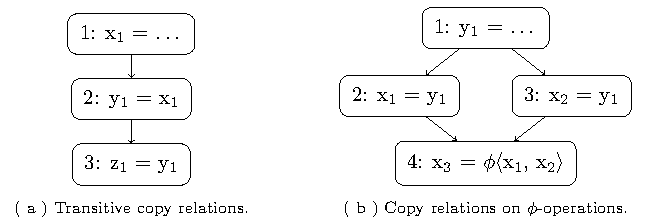
\includegraphics{copy_propagation}
    \subfigure{\label{novillo:fig:copy_propagation:a}}
    \subfigure{\label{novillo:fig:copy_propagation:b}}
  \end{center}
  \vspace{-1em}
  \caption{Analysis of copy-related variables.}
  \label{novillo:fig:copy_propagation}
\end{figure}

The analysis for copy propagation can be described as the problem of
propagating the \textit{copy-of value} of variables.  Given a sequence of
copies as shown in Figure~\ref{novillo:fig:copy_propagation:a}. We say that
y$_1$ is a \textit{copy of} x$_1$ and z$_1$ is a \textit{copy of} y$_1$.  The
problem with this representation is that there is no apparent link from z$_1$ to
x$_1$.  In order to handle transitive copy relations, all transfer functions
operate on copy-of values instead of the direct source of the copy.  If a
variable is not found to be a copy of anything else, its copy-of value is the
variable itself. For the example above, this yields that both, y$_1$ and z$_1$,
are copies of x$_1$, which in turn is a copy of itself. The lattice of this data
flow problem is thus similar to the lattice shown previously for constant
propagation. However, the lattice elements correspond to variables of the
program instead of integer numbers. The least element of the lattice
represents the fact that a variable is a copy of itself.

Similarly, we would like to obtain the result that x$_3$ is a copy of y$_1$ for
the example depicted in Figure~\ref{novillo:fig:copy_propagation:b}. This is
accomplished by choosing the meet operator such that a copy relation is
propagated whenever the copy-of values of all the $\phi$-operation's operands
match. So, when visiting the $\phi$-operation for x$_3$, the analysis finds
that x$_1$ and x$_2$ are both copies of y$_1$, which allows to propagate the
desired result that x$_3$ is a copy of y$_1$.

The following example shows a more complex situation where copy relations are
obfuscated by loops -- see Figure~\ref{novillo:fig:copy_propagation_loop}.  Note
that the actual visiting order depends on the shape of the CFG and immediate
uses, the ordering used here is meant for illustration only. Processing starts
at the operation labeled $1$, with both work lists empty and the data flow
information $\top$ associated with all variables:

\begin{figure}[t!]
  \begin{center}
    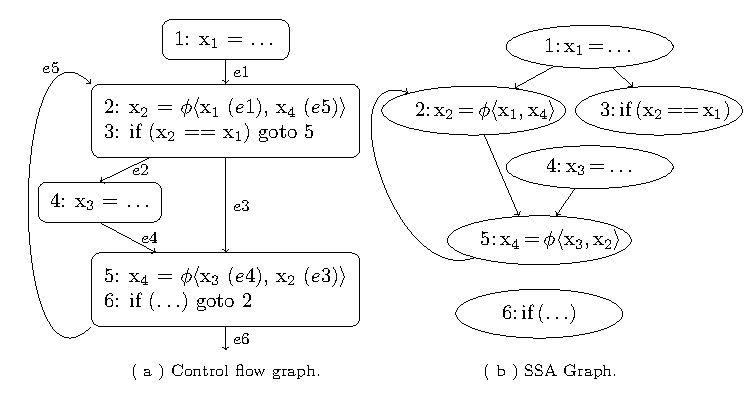
\includegraphics{copy_propagation_loop}
  \end{center}
  \vspace{-1em}
  \caption{$\phi$-operations in loops often obfuscate copy relations.}
  \label{novillo:fig:copy_propagation_loop}
\end{figure}

\begin{enumerate}
\item Assuming that the value assigned to variable x$_1$ is not a copy, the data
      flow information for this variable is lowered to $\bot$, the SSA edges
      leading to operations $2$ and $3$ are appended to the \emph{SSAWorkList},
      and the flow graph edge $e1$ is appended to the \emph{FlowWorkList}.
\item \label{novillo:copy_prop:ex:x_2} Processing the flow edge from the
      work list causes the edge to be marked executable and the operations
      labeled $2$ and $3$ to be visited. Since, edge $e5$ is not yet known to be
      executable the processing of the $\phi$-operation yields a copy relation
      between x$_2$ and x$_1$. This information is utilized in order to
      determine which outgoing flow graph edges are executable for the
      conditional branch. Examining the condition shows that only edge $e3$ is
      reachable and thus needs to be added to the work list.
\item Flow edge $e3$ is processed next and marked executable for the first time.
      Furthermore, the $\phi$-operation labeled $5$ is visited. Due to the fact
      that edge $e4$ is not known the be executable, this allows to discover a
      copy relation between x$_4$ and x$_1$ (via x$_2$). The condition of the
      branch labeled $6$ cannot be analyzed and thus causes its outgoing flow
      edges $e5$ and $e6$ to be added to the work list.
\item Now, flow edge $e5$ is processed and marked executable. Since the target
      operations are already known to be executable, only the $\phi$-operation
      is revisited. However, variables x$_1$ and x$_4$ have the same copy-of
      value x$_1$, which is identical to the previous result computed in
      Step~\ref{novillo:copy_prop:ex:x_2}. Thus, neither of the two work lists
      is modified.
\item Assuming that the flow edge $e6$ leads to the exit node of the flow graph
      the algorithm stops after processing the edge without modifications to
      the data flow information computed so far.
\end{enumerate}

The straightforward implementation of copy propagation, would have needed
multiple passes to discover that x$_4$ is a copy of x$_1$.  But the iterative
nature of the propagation along with the ability to discover non-executable
code allows to handle even obfuscated copy relations. Moreover, this kind of
propagation will only reevaluate the subset of operations affected by newly
computed data flow information instead of the complete flow graph once the set
of executable operations has been discovered.

%///////////////////////////////////////////////////////////////////////////////
\subsection{Value Range Propagation}
\label{novillo:sec:vrp}

\begin{figure}[b!]
  \begin{center}
    \begin{tabular}{c}
      \begin{lstlisting}
struct array {
  const int len;
  int *data;
};

void
doit(array *a) {
  for (int i = 0; i < a->len; ++i) {
    if (i < 0 || i >= a->len)
      throw;
    x += a->data[i];
  }
}
      \end{lstlisting}
    \end{tabular}
  \end{center}
  \caption{Useless array bound checking code.}
  \label{novillo:fig:vrp-1}
\end{figure}

\begin{figure}[t!]
  \vspace{-1em}
  \begin{center}
    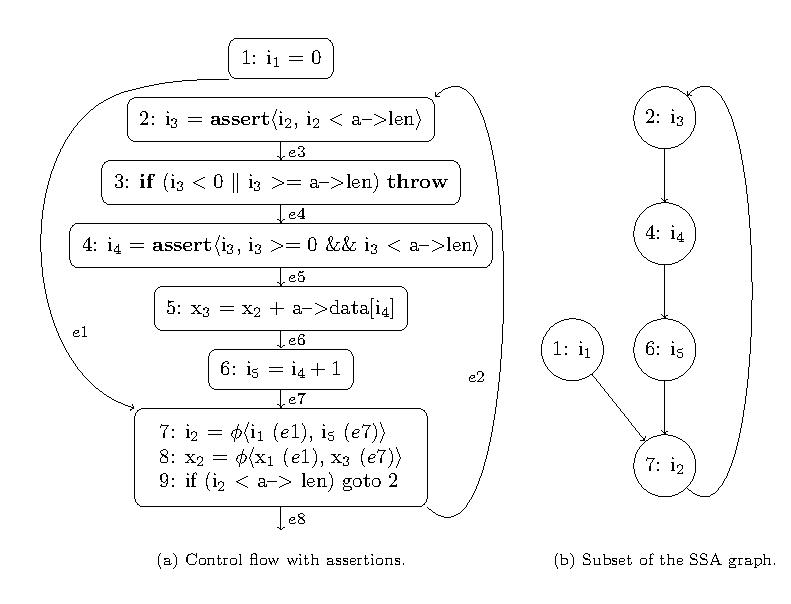
\includegraphics{value_range_propagation}
  \end{center}
  \vspace{-2em}
  \caption{Splitting live ranges using additional \emph{assert} expressions
           allows to derive more precise value ranges.}
  \subfigure{\label{novillo:fig:vrp-2:a}}
  \subfigure{\label{novillo:fig:vrp-2:b}}
  \label{novillo:fig:vrp-2}
\end{figure}

Value range propagation is similar to constant propagation, which served as a
running example throughout this chapter. But instead of propagating single
constant values, contiguous value ranges are propagated for all variables. For
instance, the code in Figure~\ref{novillo:fig:vrp-1} is extracted from a
typical expansion of bound checking code in languages like Java. Notice how the
bounds check at line $9$ is redundant as variable $i$ is guaranteed to take
values in the range [$0$, a-\textgreater len - 1]. An important source for range
information are the conditions of branch operations, e.g., the condition
associated with the \textbf{for} loop in the example.

Regular SSA graphs do not allow to take advantage of these conditions, because
the range information only applies to the code region that is guarded by the
respective branch. Furthermore, certain operations allow to derive range
information as a side effect. Typical examples are arithmetic operations with
implicit conditions such as the \emph{minimum}, \emph{maximum}, or the
\emph{absolute} operations. Trapping operations also provide information in case
the execution succeeds, e.g., a pointer is known not to be \texttt{NULL} when a
memory access succeeds. However, not all program points where this additional
range information is available are captured by SSA graphs, which capture
variable definitions, their uses, and $\phi$-operations only.

The graph is thus preprocessed in order to split the live ranges of variables
at appropriate program points whenever range information can be derived. The
splitting can be accomplished by inserting artificial \emph{assert} operations
into the SSA graph that take an input variable and a condition as operands and
return a copy of the input variable's value. Note that this \emph{ad hoc} form
of live range splitting could be generalized, e.g., by program representations
such as \emph{static single information}
(SSI)~\cite{novillo:bib:A99,novillo:bib:S05} or Extended SSA
($e$-SSA)~\cite{novillo:bib:BGV00} form -- also see Chapter~\ref{} of this
book. \obacht{Reference}{Missing reference to live range splitting chapter.}

Following this live range splitting, a data flow problem is solved in order to
propagate the range information available through the conditions of the assert
expressions to the respective uses. The lattice representing the range
information is more complex in structure than the previous examples. The lattice
elements are divided into two classes, \emph{regular} ranges and \emph{anti}
ranges, and consist of a lower and upper bound, where the bounds can be
arbitrary symbolic expressions. Regular ranges specify that the actual values of
a variable lie within the lower and upper bound, while for anti ranges the
opposite is true. The meet operator is defined by combining the bounds such that
the resulting range covers both of its arguments, i.e., in the case of regular
ranges combining the information of $r_1 = [l_1, u_1]$ and $r_2 = [l_2, u_2]$
yields the range $[min(l_1, l_2), max(u_1, u_2)]$.

However, a naive formulation of the lattice quickly leads to long or even
infinite chains. The lattice thus needs to be restricted in order to guarantee
termination of the analysis. As an example, consider a loop with an
unconditional increment of a counter variable. This could lead to an infinite
feedback look where the value range associated with the counter grows infinitely
on every iteration of the work list algorithm. In practice, infinite chains are
prevented by choosing the transfer functions such that growth is restricted. For
example, the popular open source compiler GCC, restricts the transfer functions
of many operations, such as addition or subtraction, to constant singleton
ranges only, i.e., ranges that consist of a single element that is known to be
constant. Other compiler allow the range to grow within certain limits.

The augmented CFG of the original program from Figure~\ref{novillo:fig:vrp-1} is
shown in Figure~\ref{novillo:fig:vrp-2:a}. Two additional \emph{assert}
expressions were inserted. The first, immediately following the conditional
branch of the \textbf{for} loop, while the other is placed after the bounds
check. For this example we are only interested in the value range of the counter
variable i -- and the corresponding variables in SSA form.
Figure~\ref{novillo:fig:vrp-2:b} thus only shows a subset of the complete SSA
graph that is relevant for the counter variable. In the following the major
steps of the data flow analysis are discussed:
\begin{enumerate}
\item \label{novillo:vrp:ex:i_1} The algorithm starts with the data flow
      information $\top$ assigned to all variables and by processing the
      operation labeled 1. The analysis derives the range $[0,0]$ for variable
      i$_1$, which causes the $\phi$-operations and the branch labeled $7$-$9$
      to be evaluated.
\item Since the flow edge $e7$ is not yet known to be executable the analysis
      derives the same range, $[0, 0]$, for variable i$_2$ of $\phi$-operation
      $7$.
\item Analyzing the condition of the branch operation $9$ yields that both
      outgoing edges are executable, which triggers the analysis of the
      operations within the loop.
\item At first, however, examining the conditions of the \emph{assert}
      expressions does not provide interesting ranges. The analysis merely
      retains the range $[0, 0]$ for both variables i$_3$ and i$_4$.
\item \label{novillo:vrp:ex:i_5} The analysis eventually reaches the increment
      of the counter variable labeled $6$. As mentioned before, the transfer
      function for such increments has a huge impact on the quality of the
      analysis results and worst case complexity. For the sake of simplicity,
      assume that the increment is handled conservatively. The transfer function
      yields the range $[0, \infty]$ for variable i$_5$.\footnote{Note that
      actual compilers have to assume a potential overflow of the counter
      variable, which further complicates the task of finding a proper transfer
      function.}
\item Due to the updated range information of i$_5$ and the fact that the flow
      edge $e7$ is now known to be executable, the $\phi$-operation of i$_2$ has
      to be reevaluated. Combining the range information computed by
      step~\ref{novillo:vrp:ex:i_1} and \ref{novillo:vrp:ex:i_5} yields a new
      range $[0, \infty]$.
\item Note that at this point all flow edges have been marked executable, the
      following processing steps operate on the sparse SSA graph representation
      only and thus bypass unrelated computations.
\item \label{novillo:vrp:ex:i_3} First, the \emph{assert} expression for
      variable i$_3$ is reevaluated. This time the expression's condition allows
      to clip the range of the input variable i$_2$ since the value of a-$>$len
      is known to be smaller than $\infty$. The new range for i$_3$ is thus
      $[$0, a-$>$len$ - 1]$, which triggers the reevaluation of all its uses,
      in particular the array bounds check labeled with the number $3$.
\item The second \emph{assert} expression is handled similarly and yields the
      same range, $[$0, a-$>$len$ - 1]$, for variable i$_4$. Again all of its
      uses are reevaluated.
\item Finally, the counter increment is reevaluated, however, the range for its
      variable i$_5$ does not change and the analysis terminates.

\end{enumerate}

The final result of the analysis is used in order to eliminate array bounds
checks, conditional branches, or unreachable code~\cite{novillo:bib:BGV00}. For
example, the analysis result computed at Step~\ref{novillo:vrp:ex:i_3} for the
previous example, allows to safely eliminate the array bounds check.
Furthermore, range information is valuable during the optimization of data
representations, e.g., to reduce the number of bits for certain computations
without loss of precision~\cite{novillo:bib:SBA00}.


%%%%%%%%%%%%%%%%%%%%%%%%%%%%%%%%%%%%%%%%%%%%%%%%%%%%%%%%%%%%%%%%%%%%%%%%%%%%%%%%
\section{Beyond Sparse Data Propagation}
\label{novillo:sec:beyond_sparse_data_propagation}

We have seen that the generic propagation engine is capable to elegantly solve
forward problems based on the sparse SSA graph. However, due to limitations of
the graph, not all problems can be modeled.  This section will highlight some
problems where SSA form has proven helpful using specialized algorithms.

%...............................................................................
\subsubsection*{Dead Code Elimination}

Dead code elimination (DCE) is a very important compiler optimization that
eliminates computations that do not have any effect on the program output. This
situation may arise from different sources. Code is called \emph{unreachable}
when it can never, under any circumstances, be executed at run-time. A common
case of unreachable code is often related to conditional branches where the
condition always evaluates to either true or false -- the respective other case
is unreachable, provided no other control path leads to the code.  Another form
of dead code arises from reachable computations, i.e., it is possible that the
computations are carried out at run-time, that are never used by any subsequent
computations. Dead or unreachable code can be removed in either case without
impairing the program's correctness.

A popular algorithm for DCE, a typical backward data flow analysis, is due to
Cytron et al.~\cite{novillo:bib:cytron.ea-91}. This algorithm exploits SSA form in
order to eliminate both forms of dead code. It proceeds by initially marking all
computations of a procedure to be dead. Computations are iteratively marked to
be live using a work list algorithm according to the following criteria: (1)
computations with observable side-effects such as I/O operations, function
calls, and assignments to global or shared memory locations, (2) assignments to
variables that are used by other live computations, (3) conditional branches
where at least on control-dependent computation has been marked live. When the
work list drains, no additional live computations can be discovered. The
remaining code marked as dead can safely be eliminate. It is easy to see that
SSA form simplifies the processing of criteria (2) of this algorithm, since the
relation between definitions and uses is captured naturally.

%...............................................................................
\subsubsection*{Live Variables}

Another important problem is the computation of live variables at all program
points of a procedure or a subset thereof, which is usually solved using a
backward data flow analysis. The approach is applicable to programs in SSA form,
however, due to the increased number of variable names due to renaming during
SSA construction, a considerable overhead is induced.

\obacht{Reference}{Missing reference to liveness chapter.}
Fortunately, the live ranges, i.e., the set of program points where variables
are live, offer properties under SSA form that facilitate the computation of
liveness information. In fact, several options exist that allow to derive
traditional liveness sets, where every program point is annotated with a set of
live variables, or to perform on-demand liveness checks for individual
variables~\cite{novillo:bib:BHGD08}. In either case, the fact that uses of a
variables are in any case dominated by its definition is exploited, which allows
to prune the set of program point where variables are possibly live. We do not
present details of these approaches and the involved algorithms, since
Chapter~\ref{} covers this topic in great detail.

%%%%%%%%%%%%%%%%%%%%%%%%%%%%%%%%%%%%%%%%%%%%%%%%%%%%%%%%%%%%%%%%%%%%%%%%%%%%%%%%
\section{Further Reading}
\label{novillo:sec:further_reading}

Traditional data flow analysis is well established and well described in
numerous papers. The book by Nielsen, Nielsen, and
Hankin~\cite{novillo:bib:NNH99} gives an excellent introduction to the
theoretical foundations and practical applications.

The sparse propagation engine, as presented in the chapter, is based on the
underlying properties of SSA form. Other intermediate representations offer
similar properties. \emph{Static Single Information} (SSI)
form~\cite{novillo:bib:S05} allows both backward and forward problems to be
modeled by introducing $\sigma$ operations, which are placed at program points
where data flow information for backward problems needs to be
merged~\cite{novillo:bib:S04}. Bod\'{\i}k uses an extended SSA form, $e$-SSA,
in order to eliminate array bounds checks~\cite{novillo:bib:BGV00}.
Ruf~\cite{novillo:bib:R95} introduces the \emph{value dependence graph}, which
captures both control and data dependencies. Using a set of transformations and
simplifications a sparse representation of the input program can be derived
which is suited for data flow analysis.

The \emph{sparse evaluation graph} by Choi~et.al~\cite{novillo:bib:CCF91} is
based on the same basic idea as the approach presented in this chapter,
intermediate steps are eliminating by by-passing irrelevant CFG nodes and
merging the data flow information only when necessary. Their approach is closely
related to the placement of $\phi$-operations and similarly relies on the
dominance frontier during construction. A similar approach, presented by Johnson
and Pingali~\cite{novillo:bib:JO93}, is based on single-entry/single-exit
regions. The resulting graph is usually less sparse, but is also less complex to
compute. Ramalingam~\cite{novillo:bib:R02} further extends these ideas and
introduces the \emph{compact evaluation graph}, which is constructed from the
initial CFG using two basic transformations. The approach is superior to the
sparse representations by Choi~et.al as well as the approach presented by
Johnson and Pingali.

The previous approaches derive a sparse graph suited for data flow analysis
using graph transformations applied to the CFG.
Duesterwald~et.al~\cite{novillo:bib:DGS94} instead examine the data flow
equations, eliminate redundancies, and apply simplifications to them.

